

\tikzset{every picture/.style={line width=0.75pt}} %set default line width to 0.75pt        

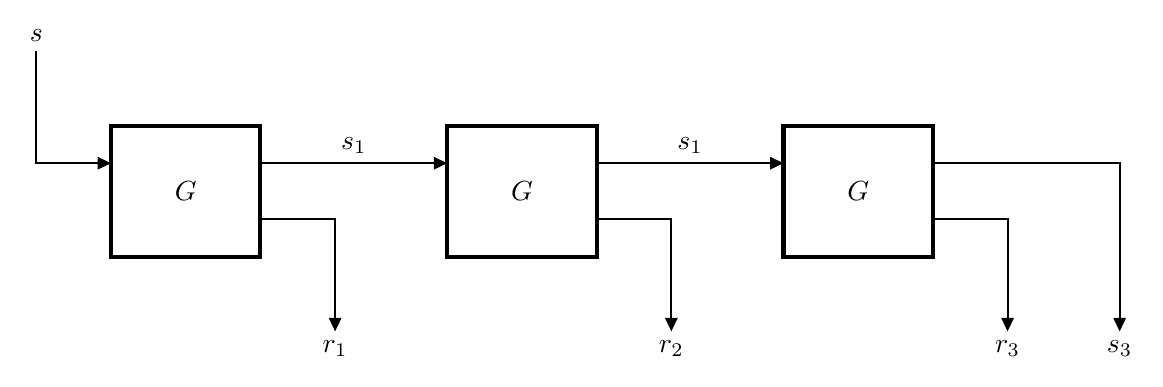
\begin{tikzpicture}[x=0.75pt,y=0.75pt,yscale=-0.9,xscale=0.9]
%uncomment if require: \path (0,188); %set diagram left start at 0, and has height of 188

%Shape: Rectangle [id:dp2160048926916731] 
\draw  [line width=1.5]  (60,40) -- (140,40) -- (140,110) -- (60,110) -- cycle ;
%Straight Lines [id:da3825330167869643] 
\draw    (20,0) -- (20,60) -- (57,60) ;
\draw [shift={(60,60)}, rotate = 180] [fill={rgb, 255:red, 0; green, 0; blue, 0 }  ][line width=0.08]  [draw opacity=0] (7.14,-3.43) -- (0,0) -- (7.14,3.43) -- cycle    ;
%Shape: Rectangle [id:dp6626895390318233] 
\draw  [line width=1.5]  (240,40) -- (320,40) -- (320,110) -- (240,110) -- cycle ;
%Shape: Rectangle [id:dp901636654927154] 
\draw  [line width=1.5]  (420,40) -- (500,40) -- (500,110) -- (420,110) -- cycle ;
%Straight Lines [id:da4691364373293083] 
\draw    (140,60) -- (237,60) ;
\draw [shift={(240,60)}, rotate = 180] [fill={rgb, 255:red, 0; green, 0; blue, 0 }  ][line width=0.08]  [draw opacity=0] (7.14,-3.43) -- (0,0) -- (7.14,3.43) -- cycle    ;
%Straight Lines [id:da5743815657646101] 
\draw    (320,60) -- (417,60) ;
\draw [shift={(420,60)}, rotate = 180] [fill={rgb, 255:red, 0; green, 0; blue, 0 }  ][line width=0.08]  [draw opacity=0] (7.14,-3.43) -- (0,0) -- (7.14,3.43) -- cycle    ;
%Straight Lines [id:da4042760753093215] 
\draw    (500,60) -- (600,60) -- (600,147) ;
\draw [shift={(600,150)}, rotate = 270] [fill={rgb, 255:red, 0; green, 0; blue, 0 }  ][line width=0.08]  [draw opacity=0] (7.14,-3.43) -- (0,0) -- (7.14,3.43) -- cycle    ;
%Straight Lines [id:da6774309103002059] 
\draw    (140,90) -- (180,90) -- (180,147) ;
\draw [shift={(180,150)}, rotate = 270] [fill={rgb, 255:red, 0; green, 0; blue, 0 }  ][line width=0.08]  [draw opacity=0] (7.14,-3.43) -- (0,0) -- (7.14,3.43) -- cycle    ;
%Straight Lines [id:da26270938097623087] 
\draw    (320,90) -- (360,90) -- (360,147) ;
\draw [shift={(360,150)}, rotate = 270] [fill={rgb, 255:red, 0; green, 0; blue, 0 }  ][line width=0.08]  [draw opacity=0] (7.14,-3.43) -- (0,0) -- (7.14,3.43) -- cycle    ;
%Straight Lines [id:da12969764248165716] 
\draw    (500,90) -- (540,90) -- (540,147) ;
\draw [shift={(540,150)}, rotate = 270] [fill={rgb, 255:red, 0; green, 0; blue, 0 }  ][line width=0.08]  [draw opacity=0] (7.14,-3.43) -- (0,0) -- (7.14,3.43) -- cycle    ;

% Text Node
\draw (20,-3.4) node [anchor=south] [inner sep=0.75pt]    {$s$};
% Text Node
\draw (100,75) node    {$G$};
% Text Node
\draw (280,75) node    {$G$};
% Text Node
\draw (460,75) node    {$G$};
% Text Node
\draw (190,56.6) node [anchor=south] [inner sep=0.75pt]    {$s_{1}$};
% Text Node
\draw (370,56.6) node [anchor=south] [inner sep=0.75pt]    {$s_{1}$};
% Text Node
\draw (180,153.4) node [anchor=north] [inner sep=0.75pt]    {$r_{1}$};
% Text Node
\draw (360,153.4) node [anchor=north] [inner sep=0.75pt]    {$r_{2}$};
% Text Node
\draw (540,153.4) node [anchor=north] [inner sep=0.75pt]    {$r_{3}$};
% Text Node
\draw (600,153.4) node [anchor=north] [inner sep=0.75pt]    {$s_{3}$};


\end{tikzpicture}